\documentclass[10pt,a4paper]{article}
\usepackage[latin1]{inputenc}
\usepackage[spanish]{babel}
\usepackage{amsmath}
\usepackage{amsfonts}
\usepackage{amssymb}
\usepackage{xcolor,color}
\usepackage{graphicx}
\addcontentsline{toc}{chapter}{Bibliograf�a}
\usepackage{tikz}

\usepackage{enumitem}
\newcommand*{\itembolasazules}[1]{% bolas 3D
\footnotesize\protect\tikz[baseline=-3pt]%
\protect\node[scale=.7, circle, shade, ball
   color=blue]{\color{white}\Large\bf#1};}


\usepackage[left=4cm,right=3cm,top=4cm,bottom=3cm]{geometry}
\author{Enrique QC}
\title{Distribucion  Muestral}


%caratula
\begin{document}
\begin{center}
\LARGE\bf{UNIVERSIDAD NACIONAL SAN CRISTOBAL DE  HUAMANGA}
\end{center}
\begin{center}
\Large\bf{FACULTAD DE  ING. DE MINAS, GEOLOGIA Y CIVIL}
\end{center}
\begin{center}
\small\bf{ESCUELA PROFESIONAL INGENIERIA DE SISTEMAS}
\end{center}
\begin{center}

\includegraphics[width=3.5cm]{logo.jpg}  
\end{center}

\begin{center}
\textbf{ {\large \textit{\underline{{\small DISTRIBUCION MUESTRAL DE LA MEDIA}}}}}
\end{center}
\textbf{ASIGNATURA }\quad\quad\quad\quad{: ESTADISTICA II  (ES - 244)}\\\\
\textbf{SERIE }\quad\quad\quad\quad\quad\quad\quad\quad\quad{: 200}\\\\
\textbf{CREDITO }\quad\quad\quad\quad\quad\quad\quad{: 4}\\\\
\textbf{SEMESTRE}\quad\quad\quad\quad\quad\quad{: 2019-II}\\\\

\textbf{INTEGRANTES}: \\ 
\begin{enumerate}[label=\itembolasazules{\arabic*}]
   \item QUISPE\quad CUCHURI, Enrique
   \item BARZOLA\quad YUPANQUI, Mardonio
   \item VERA\quad PALOMINO, Sirlhey
   \item LIZANA\quad GUEVARA, Raquel
   \\\\
\end{enumerate}
\textbf{DOCENTE}: ROMERO PLASENCIA, Jackson M'coy \\
\\
\begin{center}
\textit{Ayacucho -2019}
\end{center}

\footnote{Ingenier�a de Sistemas // \LaTeX}
%ejercicios


\newpage


\begin{center}
{\raggedright
\textbf{{\Large \underline{RESOLUCION DE EJERCICIOS}}}
}

\end{center}

\vspace{0.6cm}

{\Large Ejercicio 01.}\\
Un taller tiene 5 empleados. Los salarios diarios en dolares de cada uno de ellos son: 5,7,8,10,10.\\

a.Determinar la media y la varianza de la poblacion.\\
b.Halle la distribucion muestral de las medias para muestras de tama�o 2 escogidas (sin sustitucion) de esta poblacion.\\
c. Determine la media y la varianza de la distribucion muestral de las medidas de tama�o 2.\\
d. Compare la media de las medias muestras con la media de la poblacion. Tambien compare la dispersion de las medias de las muestras con la dispersion de la poblacion.\\\\


\textcolor {red}{\bf \fbox{SOLUCION}}

\textbf{DATOS}\\

Taller con 5 empleados

salario diario c/u 5, 7, 8, 10, 10\\

A) Media Poblacional\\
${ { \mu =\frac { \sum _{ i=1 }^{ 5 }{ { x }_{ i } }  }{ 5 } ={ \frac { { x }_{ 1 }+x_{ 2 }+{ x }_{ 3 }+{ x }_{ 4 }+{ x }_{ 5 } }{ 5 }  } } }$\\\\

 
$\frac { { 5+7+8+10+10 }{ \quad  } }{ 5 } =8$\\\\
 
$\mu=8$\\

\fcolorbox{orange}{gray}{ \color{black} $\therefore \mu=8$}\\\\

Varianza poblacional\\ 
${ \sigma  }^{ 2 }=\dfrac { \sum _{ i=1 }^{ N }{ { ({ x }_{ i }-\mu ) }^{ 2 } }  }{ N }$ \\ 

tomamos el promedio de las distancias al cuadrado\\

 ${ \sigma  }^{ 2 }=\dfrac { { (5-8) }^{ 2 }+{ (7-8) }^{ 2 }+{ (8-8) }^{ 2 }+{ (10-8) }^{ 2 }+{ (10-8) }^{ 2 } }{ 5 }$ \\\\
 
 ${ \sigma  }^{ 2 }=\dfrac { 9+1+0+4+4 }{ 5 } =\quad 3.6$\\\\ 

${\sigma  }^{ 2 }= =\quad 3.6$\\

\fcolorbox{orange}{gray}{ \color{black} $\therefore {\sigma  }^{ 2 }=\quad 3.6$}\\\\

B)Posibles muestras de tama�o dos extrai�dos de una poblacion finita de tama�o cinco.\\ 
$(5,7),(5,8),(5,10),(5,10)\qquad \qquad 4\quad muestras$\\ 
$(7,8),(7,10),(7,10)\qquad \qquad \qquad 3\quad muestras$\\ 
$(8,10),(8,10)\qquad \qquad \qquad \qquad 2\quad muestras$\\ 
$(10,10)\qquad \qquad \qquad \qquad \qquad 1\quad muestra$\\

Aplicando la Formula de combinacion se tiene el mismo resultado\\
 
${ nCr=n!/r!(n-r)!}$\\\\
  
 
$\dfrac {5!}{2!(5-2)!} =\dfrac {5x4x3!}{2!x3!} =10$\\\\
  
\begin{center}
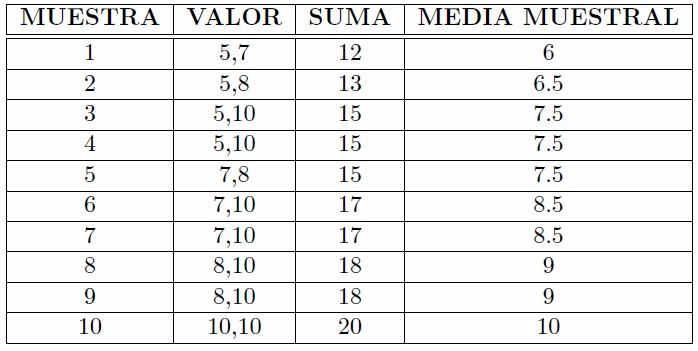
\includegraphics[width=10cm]{d1.JPG} 
\end{center}

\begin{center}
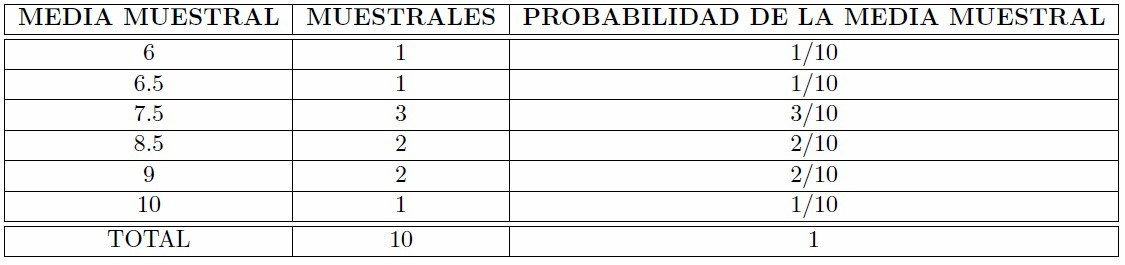
\includegraphics[width=15cm]{d2.JPG} 
\end{center}

D)Media aritmetica de la distribucion muestral de la media:\\


${ \mu =\mu }_{ \overset { - }{ x }  }$\\\\
${ { \mu  }_{ \overset { - }{ x }  }=8 }$\\\\

Desviacion estandar de la distribucion de la media \\
${ { \theta  }_{ \overset { - }{ x }  }^{ 2 }=\frac { { \theta  }^{ 2 } }{ \sqrt { 2 }  } x\sqrt { \frac { N-2 }{ N-1 }  }  }$\\\\

${ \theta  }_{ \overset { - }{ x }  }^{ 2 }=\frac { 3.6 }{ \sqrt { 2 }  } x\sqrt { \frac { 5-2 }{ 5-1 }  } =1.349999$ \\\\



{\Large Ejercicio 02.}\\
De la historia sacada de los registros de a universidad sea determinado que las calificaciones del curso de MATE1 y de FILO1 se distribuyen normalmente con las medidas respectivas 12 y 15 y con varianzas homogeneas igual a 4. �Cual es la probabilidad de que la media de las notas de un alumno que llevo tales cursos esta entre 13 y 16?\\\\

\textcolor {red}{\bf \fbox{SOLUCION}}\\

media de la muestra\\
$\mu =\frac { \sum _{ i=1 }^{  }{ { x }_{ i } }  }{ n }$ \\\\
$\frac { 12+15 }{ 2 } \quad =\quad 13.5$\\\\


variacion de la muestra
${ \sigma  }^{ 2 }=\frac { \sum _{ i=1 }^{ n }{ { ({ x }_{ i }-\mu ) }^{ 2 } }  }{ n } $\\\\
${ \sigma  }^{ 2 }=\frac { { (12-13.5) }^{ 2 }+{ (15-13.5) }^{ 2 } }{ 2 }$\\\\ 
${ \sigma  }^{ 2 }=\quad 2.25$\\\\
${ \sigma  }=\sqrt { 2.25 } =\quad 1.5$\\\\


$P(13<\overline { X } <16)$\\\\ $P(\frac { \overline { X } -\mu  }{ \sigma  } <Z<\frac { \overline { X } -\mu  }{ \sigma  } )$\\\\ $P(\frac { 13-13.5 }{ 1.5 } <Z<\frac { 16-16.5 }{ 1.5 } )$\\\\ $P(-0.333<Z<1.666)$\\\\ $=P(Z<1.666)-P(Z<-0.333)$\\\\ $=0.95154-\left[ 1-0.62930 \right] $\\\\ $=0.58084$

\fcolorbox{orange}{gray}{ \color{black} $\therefore 0.58084$}\\\\



{\Large Ejercicio 03.}\\
Si\quad $\overline { X } $\quad denota\quad una\quad media\quad de\quad la\quad muestra\quad aleatoria\quad ${ X }_{ 1 },{ X }_{ 2 },{ X }_{ 3 },...,{ X }_{ 9 }$\quad de\quad tam�o\quad 9\quad escogida\quad de\quad la\quad poblacion\quad $(X)$\quad normal\quad $N(6,6^{ 2 })$.\\\\

 A).\quad Halle\quad el\quad percentil\quad 80\quad de\quad la\quad distribucion\quad de\quad la\quad distribucion\quad de\quad $\overline { X } $.\\\\ 
 
 B).\quad Si\quad $Y=3X-5$,\quad calcular\quad $P\left[ \overline { Y } >28 \right] $.\\\\

\textcolor {red}{\bf \fbox{SOLUCION}}\\


$n=9; X \longrightarrow N(6,6^{ 2 }) $

A). ${ P }_{ 80 }=?$\\

${ P }(X\le k)=0.80$\\\\ 
$P(\frac { X-\mu  }{ \frac { \sigma  }{ \sqrt { n }  }  } \le \frac { k-6 }{ \frac { 6 }{ \sqrt { 9 }  }  } )=0.80$\\\\ 
$P(Z\le \frac { k-6 }{ 2 } )=0.80$\\\\ 
$F(z)\Longrightarrow 0.85$\\\\ $\frac { k-6 }{ 2 } =0.85\Longrightarrow k=7.7$\\

\fcolorbox{orange}{gray}{ \color{black} $\therefore k=7.7$}\\\\

B). $y=3x-5$\\\\ $E(y)=E(3x-5)$\\\\ $=3E(x)-E(5)$\\\\ $=3\mu -5=3(6)-5=13$\\\\ $E(y)=13$\\ \\ $Var(y)=Var(3x-5)$\\ $=9Var(x)+0$\\\\ $=9(36)=324$\\\\ $Var(y)=324$\\\\ ${ P }(Y>28)=1-P(\frac { Y-\mu  }{ \frac { \sigma  }{ \sqrt { n }  }  } \le \frac { 28-13 }{ \frac { 18 }{ \sqrt { 9 }  }  } )$\\\\ $=1-P(Z\le 2.5)$\\\\ $=1-0.99379$\\\\ $=0.00621$\\\\

\fcolorbox{orange}{gray}{ \color{black} $\therefore 0.00621$}\\\\

{\Large Ejercicio 05.}\\
La demanda diaria de un producto puede ser :0,1,2,3,4 con probabilidades respectivas: 0.3,0.3,0.2,0.1,0.1.
A). Describa el modelo de probabilidad de la demanda promedio de 36 dias.
B).�Que probabilidad hay de que la demanda promedio de 36 dias este entre 1 y2 inclusive?.\\

\textcolor {red}{\bf \fbox{SOLUCION}}\\

$X:\quad Demanda\quad diaria\quad de\quad un\quad producto$\\ 
a)  $n=36$ \\\\
${ \quad { \mu  }_{ x }=\quad E(x)=\quad \sum { xp(x)=0(0.3)+1(0.3)+2(0.2)+3(0.1)+4(0.1) }  }$\\\\
${ \mu  }_{ x }=1.4$\\\\ 
${ E({ x }^{ 2 })=\sum { { x }^{ 2 } } p(x)={ 0 }^{ 2 }(0.3)+{ 1 }^{ 2 }(0.3)+{ 2 }^{ 2 }(0.2)+{ 3 }^{ 2 }(0.1)+{ 4 }^{ 2 }(0.1) }$\\\\ 
$E({ x }^{ 2 })=3.6$\\\\ 
$VAR(x)\quad =\quad E({ x }^{ 2 })-{ \mu  }^{ 2 }$\\\\ 
${ \sigma  }_{ x }^{ 2 }\quad =\quad 3.2-{ 1.4 }^{ 2 }$\\\\ 
${ \sigma  }_{ x }\quad =\quad 0.045$\\\\
 
b)$P(-1\le x\le Z)\quad =\quad \phi \quad (\frac { 2-1.4 }{ 0.21343 } )\quad -\quad \phi \quad (\frac { 1-1.4 }{ 0.21343 } )$\\\\ 
$=\quad \phi \quad (2.81)\quad -\quad \phi \quad (-1.87)$\\\\ 
 $=\quad \phi \quad (2.81)\quad -\quad [1-\quad \phi \quad (1.87)]$\\\\
$=\quad 0.9668$\\\\

{\Large Ejercicio 06.}\\
Una empresa comercializadora de cafe sabe que el consumo mensual en kilogramos de caf� por casa esta normalmente distribuida con una media desconocida $\mu $ y la desviacion estandar de 0.30. Si se toma una muestra aleatoria de 36 casas y se registra su consumo de cafe durante un mes. �Cual es �a probabilidad de que  la media  de la muestra este entre los valores $\mu -1$ y $\mu +1$?\\
\textcolor {red}{\bf \fbox{SOLUCION}}\\

$\mu =?\quad ,\quad \sigma =0.30\quad ,\quad n=36$\\\\ 
$P(\mu -0.1<\overline { X } <\mu +0.1)$\\\\ 
$P(\frac { \mu -0.1-\mu  }{ \frac { 0.30 }{ \sqrt { 36 }  }  } <Z<\frac { \mu +0.1-\mu  }{ \frac { 0.30 }{ \sqrt { 36 }  }  } )$\\\\ 
$P(-2<Z<2)$\\\\ $P(Z<2)-P(Z<-2)=0.97725-\left[ 1-0.97725 \right] $\\\\ 
$=0.9545$\\

\fcolorbox{orange}{gray}{ \color{black} $\therefore 0.9545$}\\



{\Large Ejercicio 07.}\\ 
La distribucion de las notas del examen final de Mat.I resulto ser normal  
$N(\mu ,{\sigma}^{ 2 })$, los cuartiles 1 y 3 iguales a 6.99 y 10.01 respectivamente.

a.-Determine\quad la\quad media\quad y\quad la\quad varianza\quad de\quad la\quad distribucion\quad de\quad las\quad notas.\\ 

b.-Halle el intervalo $[a,b]$  centrado en $\mu $ tal que $P\left[ a\le \overline { x } \le b \right] =0.9544$, donde $\overline { x }$ es la media de la muestra ${ x }_{ 1 },{ x }_{ 2 },{ x }_{ 3 },{ x }_{ 4 }\quad escogida\quad de\quad esa\quad poblacion$.\\
 
\textcolor {red}{\bf \fbox{SOLUCION}}
 
{\bf a).} 
$N\left( \mu ,{ \sigma  }^{ 2 } \right) $\\\\ ${ Q }_{ 1 }=6.99={ P }_{ 25 }$\\\\ ${ Q }_{ 3 }=11.01={ P }_{ 75 }$\\\\ ${ Q }_{ 2 }=\frac { { { Q }_{ 1 }+Q }_{ 3 } }{ 2 } =9$\\\\ $\quad \Rrightarrow \quad { \mu  }_{ \overline { x }  }=9$\\\\

$P\left( \overline { X } \le 6.99 \right) =0.25$\\\\ $P\left( Z\le \frac { 6.99-9 }{ \sigma  }  \right) =0.25$\\\\ $Z=-0.68=\frac { 6.99-9 }{ \sigma  } $\\\\ $\Rrightarrow \sigma =3$\\

\fcolorbox{orange}{gray}{ \color{black} $\therefore \quad\sigma =3$}\\
 
{\bf b).} 
$P(a\le \overline { X } \le b)=0.9544$\\\\ 
$P(\overline { X } \le b)-P(\overline { X } \le a)=0.9544$\\\\ 
$P(Z\le \frac { b-\mu  }{ \frac { \sigma  }{ \sqrt { n }  }  } )-P(Z\le \frac { a-\mu  }{ \frac { \sigma  }{ \sqrt { n }  }  } )=0.9544$\\\\
 
$P(Z\le \frac { b-\mu  }{ \frac { \sigma  }{ \sqrt { n }  }  } )-\left[ 1-P(Z\le \frac { a-\mu  }{ \frac { \sigma  }{ \sqrt { n }  }  }  \right] )=0.9544$\\\\
$2P(Z\le \frac { b-\mu  }{ \frac { \sigma  }{ \sqrt { n }  }  } )-1=0.9544$\\\\
$P(Z\le \frac { b-\mu  }{ \frac { \sigma  }{ \sqrt { n }  }  } )=0.9772$\\\\ 
$Z=2=\frac { b-\mu  }{ \frac { \sigma  }{ \sqrt { n }  }  } =\frac { b-9 }{ \frac { 3 }{ 2 }  } ,\quad \Rrightarrow \quad b=12\quad \Longrightarrow \quad \frac { a-9 }{ \frac { 3 }{ 2 }  } =-2\quad \Longrightarrow \quad a=6$\\\\ 

\fcolorbox{orange}{gray}{ \color{black} $\therefore \quad b=12\quad \quad y\quad a=6 $}\\ 

{\Large Ejercicio 08.}\\
La\quad vida\quad util\quad (en\quad miles\quad de\quad horas)\quad de\quad una\quad bateria\quad es\quad una\quad variable\quad aleatoria\quad con\quad funcion\quad de\quad densidad:\\

\[f(x)=\left\{ \begin{array}{rcl}
2-2x & , & 0\le x \le 1\\
& & \\
0 &, en \quad el \quad resto \\
\end{array}
\right. \]

Si\quad ${ \overline { X }  }_{ 36 }$\quad es\quad la\quad medida\quad de\quad una\quad muestra\quad aleatoria\quad ${ x }_{ 1 },{ x }_{ 2 },{ x }_{ 3 },{ x }_{ 4 },...{ ,x }_{ 36 }$\quad escogida\quad de\quad X.\\

�Con\quad que\quad probabilidad\quad ${ \overline { X }  }_{ 36 }$\quad \quad es\quad mayor\quad que\quad 420\quad horas?\\

\textcolor {red}{\bf \fbox{SOLUCION}}

$X:$\quad vida\quad util\quad (1000\quad horas)\\\\ 
$f\left( x \right) =2-2x,\quad 0\quad \le x\le 1$\\\\ 
$\int _{ 0 }^{ 1 }{ f\left( x \right) =1\quad  } \Rightarrow \quad \int _{ 0 }^{ 1 }{ \left( 2-2x \right) dx=1\quad  } \Rightarrow \quad 2x-{ x }^{ 2 }{ | }_{ 0 }^{ 1 }\quad =2-1=1$\\\\ 
${ \sigma  }^{ 2 }=Var(x)=E({ x }^{ 2 })-{ \left[ E(x) \right]  }^{ 2 }$\\\\
$P({ \overline { x }  }_{ 36 }>420)$\\\\ 
$P({ \overline { x }  }_{ 36 }>0.42)$\\\\ 
$\ast \mu =E(x)=\int _{ 0 }^{ 1 }{ { x }\left( 2-2x \right) dx=1\quad  } \Rightarrow \quad { x }^{ 2 }-{ \frac { 2 }{ 3 } x }^{ 2 }{ | }_{ 0 }^{ 1 }$\\\\ 
$=1-\frac { 2 }{ 3 } =\frac { 1 }{ 3 } =0.33\quad \Rightarrow \quad \therefore \mu =0.33$\\\\


$\ast E({ x }^{ 2 })=\int _{ 0 }^{ 1 }{ { x }^{ 2 }\left( 2-2x \right) dx=1\quad  } \Rightarrow \quad { \frac { 2 }{ 3 } x }^{ 2 }-{ \frac { 1 }{ 3 } x }^{ 4 }{ | }_{ 0 }^{ 1 }=\frac { 2 }{ 3 } -\frac { 1 }{ 2 } =\frac { 1 }{ 6 } $\\\\ 
${ \sigma  }^{ 2 }=Var(x)=E({ x }^{ 2 })-{ \left[ E(x) \right]  }^{ 2 }=\frac { 1 }{ 6 } -\frac { 1 }{ 9 } =\frac { 1 }{ 18 } $\\\\ 
$P(\frac { { \overline { x }  }_{ 36 }-\mu  }{ \frac { \sigma  }{ \sqrt { n }  }  } >\frac { 0.42-0.33 }{ \frac { \sqrt { \frac { 1 }{ 18 }  }  }{ \sqrt { 36 }  }  } )$\\\\ 
$P(Z>a)=1-P(Z\le a)$\\\\
$=1-P(Z\le 2.21)=1-0.98645$\\\\ 
$\quad =0.0136$

\fcolorbox{orange}{gray}{ \color{black} $\therefore \quad 0.0136 $}\\


{\Large Ejercicio 10.}\\
El\quad tiempo\quad de\quad vida\quad de\quad una\quad bateria\quad es\quad una\quad variable\quad aleatoria\quad X\quad con\quad distribucion\quad exponencial\quad de\quad parametro:\quad $1/\theta $.\quad Se\quad escoge\quad una\quad muestra\quad de\quad $n$\quad baterias.\\\\ A).\quad Halle\quad el\quad error\quad estandar\quad de\quad la\quad media\quad muestral\quad $\overline { X } $.\\\\ 
B).\quad Si\quad la\quad muestra\quad aleatoria\quad es\quad de\quad tama�o\quad $n=64$,\quad �Con\quad que\quad probabilidad\quad diferira\quad $\overline { X } $\quad del\quad verdadero\quad valor\quad \quad de\quad $\theta $\quad en\quad menos\quad de\quad un\quad error\quad estandar?\\\\ 
C).\quad �Que\quad tama�o\quad de\quad muestra\quad minimo\quad seria\quad necesario\quad para\quad la\quad media\quad muestral\quad $\overline { X } $\quad tenga\quad un\quad error\quad estandar\quad menor\quad a\quad un\quad 5 por ciento\quad del\quad valor\quad real\quad de\quad $\theta $.?\\

\textcolor {red}{\bf \fbox{SOLUCION}}

A). $X:\quad tiempo\quad de\quad vida$\\\\ 
$f(x)=\frac { 1 }{ \theta  } { e }^{ \frac { -x }{ \theta  }  }$\\\\ 
$\sqrt { var(x) } =\frac { \sigma  }{ \sqrt { n }  } \quad error\quad estandar$\\\\ $var(\overline { x } )=\frac { { \sigma  }^{ 2 } }{ n } $\\\\ 
$\mu =\int _{ 0 }^{ +\infty  }{ \frac { x }{ \theta  } { e }^{ \frac { -x }{ \theta  }  } } dx$\\\\ 
$E(x)=\mu =\theta \int _{ 0 }^{ +\infty  }{ { (\frac { x }{ \theta  } ) }^{ 2-1 }{ e }^{ \frac { -x }{ \theta  }  } } d(\frac { x }{ \theta  } )\Longrightarrow E(x)=\theta $\\\\ 
$E({ x }^{ 2 })=\int _{ 0 }^{ +\infty  }{ { x }^{ 2 } } { e }^{ \frac { -x }{ \theta  }  }d(\frac { x }{ \theta  } )={ \theta  }^{ 2 }\int _{ 0 }^{ +\infty  }{ \frac { { x }^{ 2 } }{ { \theta  }^{ 2 } }  } { e }^{ \frac { -x }{ \theta  }  }d(\frac { x }{ \theta  } )$\\\\ 
${ =\theta  }^{ 2 }\int _{ 0 }^{ +\infty  }{ { (\frac { x }{ \theta  } ) }^{ 3-1 }{ e }^{ \frac { -x }{ \theta  }  }d(\frac { x }{ \theta  } ) } \Longrightarrow E({ x }^{ 2 })=2{ \theta  }^{ 2 }$\\\\ 
${ \sigma  }^{ 2 }:\quad var(x)=2{ \theta  }^{ 2 }-\theta ={ \theta  }^{ 2 }$\\\\ $donde:\quad var(x)=\frac { { \sigma  }^{ 2 } }{ n } =\frac { \theta  }{ \sqrt { n }  } $\\

\fcolorbox{orange}{gray}{ \color{black} $\therefore \frac { \theta  }{ \sqrt { n }  }  $}\\

B). Tama�o $n=64$

$P(\overline { X } -\theta \le \sqrt { var(\overline { X } ) } )=P(\overline { X } -\theta \le \frac { \theta  }{ 64 } )=P(\overline { X } -\theta \le \frac { \theta  }{ 8 } )$\\ $P(\frac { x-8 }{ \frac { \theta  }{ \sqrt { n }  }  } \le \frac { \theta /8 }{ \theta /8 } )=P(Z\le 1)=0.68$

\fcolorbox{orange}{gray}{ \color{black} $\therefore 0.68 $}\\

C). $\frac { \theta  }{ \sqrt { n }  } <0.05\Longrightarrow \frac { 1 }{ 0.05 } <\sqrt { n } =20<\sqrt { n } \Longrightarrow n>4000$

\fcolorbox{orange}{gray}{ \color{black} $\therefore n>4000 $}\\



{\Large Ejercicio 12.}\\
La\quad vida\quad util\quad de\quad cierta\quad marca\quad de\quad llantas\quad radiales\quad es\quad una\quad variable\quad aleatoria\quad $X$\quad cuya\quad distribucion es\quad normal\quad con\quad $\mu =38.000Km$\quad y\quad $\sigma =3.000Km$.\\ A).\quad Si\quad la\quad utilidad\quad $Y$\quad (en\quad Dolares)\quad que\quad produce\quad cada\quad llanta\quad esta\quad dada\quad por\quad la\quad relacion:\\ $y=0.2x+100.$\quad �Cual\quad es\quad la\quad probabilidad\quad de\quad que\quad la\quad utilidad\quad sea\quad mayor\quad que\quad $8.900$\quad dolares?\\ B).\quad Determine\quad el\quad numero\quad de\quad tales\quad llantas\quad que\quad debe\quad adquirir\quad una\quad empresa\quad de\quad transporte\quad para\quad conseguir una\quad utilidad\quad media\quad de\quad al\quad menos\quad $7541$\quad dolares\quad con\quad probabilidad\quad $0.996$.\\\\

\textcolor {red}{\bf \fbox{SOLUCION}}

A).\quad Utilidad\quad en\quad dolares\\\\ 
$y=0.2x+100$\\\\ $E(y)=0.2E(x)+100$\\\\ $E(y)=0.2(3800)+100$\\\\ 
$E(y)=7700$\\\\ 
$Var(y)={ 0.2 }^{ 2 }Var(x)$\\\\ 
${ \sigma  }_{ y }=0.2{ \sigma  }_{ x }=0.2(3000)=600$\\\\ 
$P(y>8900)=1-P(y\le \frac { 8900-7700 }{ 600 } )$\\\\ 
$=1-P(y\le 2)$\\\\ 
$=1-09772$\\\\ 
$=0.0228$\\\\
\fcolorbox{orange}{gray}{ \color{black} $\therefore \quad 0.0228 $}\\

B).\quad $P(y>7541)=0.996$\\\\ 
$P(y>7541)=1-P(y\le \frac { 7541-7700 }{ \frac { 600 }{ \sqrt { n }  }  } )$\\\\ $0.996=1-P(y\le \frac { 7541-7700 }{ \frac { 600 }{ \sqrt { n }  }  } )$\\\\ 
$P(y\le \frac { 7541-7700 }{ \frac { 600 }{ \sqrt { n }  }  } )=0.004$\\\\ 
$\frac { 7541-7700 }{ \frac { 600 }{ \sqrt { n }  }  } =-2.65$\\\\ 
$\Rightarrow n=100$\\\\
\fcolorbox{orange}{gray}{ \color{black} $\therefore \quad n=100 $}\\

{\Large Ejercicio 13.}\\ 
Un proceso autom�tico llena bolsas de caf� cuyo peso neto tiene una media de 250 gramos y una desviaci�n estandar de 3 gramos. Para controlar el proceso, cada hora se pesan 36 bolsas escogidas al azar; si el peso neto medio esta entre 249 y 251 gramos se continua con el proceso aceptando que el peso neto medio es 250 gramos y en caso contrario, se detiene el proceso para reajustar la maquina.
A).�Cual es la probabilidad de detener el proceso cuando el peso neto medio realmente es 250?.
B).�Cual es la probabilidad de aceptar que el peso neto promedio es 250 cuando realmente es de 248 gramos?\\

\textcolor {red}{\bf \fbox{SOLUCION}}

A).$\mu =250\quad ,\quad \sigma =3\quad ,\quad n=36$\\\\
$P(249<\overline { X } )=\frac { \alpha  }{ 2 } $\\\\ 
$P(\frac { \overline { X } -\mu  }{ \frac { \sigma  }{ \sqrt { n }  }  } <\frac { 249-250 }{ \frac { 3 }{ \sqrt { 36 }  }  } )=\frac { \alpha  }{ 2 } $\\\\ 
$P(Z<-2)=\frac { \alpha  }{ 2 } $\\\\ 
Buscando\quad en\quad la\quad tabla\quad el\quad valor\quad de\quad $f(Z)$\\\\ $0.02275=\frac { \alpha  }{ 2 } $\\ $\alpha =0.456$\\\\
\fcolorbox{orange}{gray}{ \color{black} $\therefore \alpha =0.456 $}\\

B).\quad $P(\overline { X } >251)$\\\\ 
$P(Z>\frac { \overline { X } -\mu  }{ \frac { \sigma  }{ \sqrt { n }  }  } )$\\\\ $P(Z>\frac { 251-250 }{ \frac { 3 }{ \sqrt { 36 }  }  } )\quad =P(Z>2)=1-P(Z\le 2)$\\\\ 
$=1-0.9772$\\\\ 
$=0.0228$\\\\

\fcolorbox{orange}{gray}{ \color{black} $\therefore 0.0228 $}\\

{\Large Ejercicio 14.}\\
La utilidad por la venta de un cierto articulo, en miles de soles, es una variable aleatoria con distribuci�n normal. En el $5 por ciento$ de las ventas la utilidad ha sido menos que 6.71 mientras que el $1 por ciento$ de las ventas ha sido mayor que 14.66. Si se realizan 16 operaciones de ventas.�Cual es la probabilidadde que el promedio de la utilidad por cada operacion este entre 10000 y 11000 dolares?.\\

\textcolor {red}{\bf \fbox{SOLUCION}}

$si\quad x\quad es\quad la\quad variable\quad aleatoria\quad \longrightarrow \quad x\epsilon (\mu ,\sigma )$\\\\ 
$P(x<6.71)-0.05$\\\\ 
$P(x>14.66)-0.01\quad \longrightarrow \quad P(x\le 14.66)=0.99$\\\\ 
la\quad media\quad de\quad las\quad 16\quad muestras\quad de\quad x\\\\ 
$N={ N=(\mu ,\frac { \sigma  }{ 16 } ) }$\\\\ 
$P(10\quad <\quad x\quad <\quad 11)$\\\\ si\quad normalizamos\\ $P(x<6.71)-0.05$\\\\ 
$P(x>14.66)-0.01$\\\\ 
$\Rightarrow { Z=\frac { x-\mu  }{ \sigma  }  }\quad =\quad { P(Z<\frac { 6.71-\mu  }{ \sigma  } )=0.05 }$\\\\ 
${ P(Z<\frac { 14.66-\mu  }{ \sigma  } )=0.99 }$\\



{\Large Ejercicio 16.}\\
En cierta poblacion de matrimonios el peso en kilogramos de esposos y esposos se distribuye normalmente $N(80,100) y N(64,69)$ respectivamente y son independientes. Si se eligen 25 matrimonios al azar de esa poblacion calcular la probabilidad de que la media de los pesos sea a lo mas 137 Kg.\\\\ 

\textcolor {red}{\bf \fbox{SOLUCION}}

Como es una distribucion normal de peso en kilogramos, entonces la distribucion normal del peso varones y mujeres seria:$ N(144,169)$\\\\

De los datos obtenemos: $\mu = 144;\sigma^2 = 169; n = 25$\\\\

entonces:\\\\

$P(\overline{X} \leq 37)$\\\\

$P(\overline{X}-\mu / \sqrt{\frac{\sigma^{2}}{n}}\leq \frac{137-144}{\frac{13}{5}})
P(Z \leq -2.69)$\\\\

Por lo tanto la probabilidad sera: $0.0036$\\\\ 

\fcolorbox{orange}{gray}{ \color{black} $\therefore 0.0036$}\\



{\Large Ejercicio 17.}\\
Una empresa vende bloques de marmol cuyo peso se destribuye normalmente con una media de 200 kilogramos.
\\ a)Calcular la varianza del peso de los bloques, si la probabilidad de que el peso este entre 165 Kg y 235 Kg es 0.9876.
\\ b)�Que tan grande debe ser la muestra para que haya una probabilidad de 0.9938 de que el peso medio de la muestra sea inferior a 205 Kg?\\

\textcolor {red}{\bf \fbox{SOLUCION}}


Como datos se tienen: $\mu = 200 Kg$\\ 

A) Resolucion parte a:

$P(165 < X < 235)= 0.9876 $\\\\

$P(\frac{165-200}{\sigma}<Z<\frac{235-200}{\sigma}) = 0.9876$\\\\
$P(\frac{-35}{\sigma}<Z<\frac{35}{\sigma}) = 0.9876$\\\\
$P(Z<\frac{35}{\sigma})- P(Z<\frac{-35}{\sigma}) = 0.9876$\\\\
$P(Z<\frac{35}{\sigma})- (1-P(Z<\frac{35}{\sigma}))= 0.9876$\\\\
$2*P(Z<\frac{35}{\sigma}) = 1.9876$\\\\
$P(Z<\frac{35}{\sigma}) = 0.9938$\\\\
Como $f(Z)=0.9938$, entonces $Z = 2.50$.\\\\
Igualamos $\frac{35}{\sigma} = Z = 2.50$\\\\
Luego: $\sigma = 14$\\\\
\fcolorbox{orange}{gray}{ \color{black} $\therefore \sigma = 14 $}\\

B) Resolucion parte b:

$P(X < 205 ) = 0.9938$\\\\
$P(\frac{X -\mu}{\frac{\sigma}{\sqrt{n}}}<\frac{201-200}{\frac{14}{\sqrt{n}}}) = 0.9938$\\\\
$P(Z<\frac{5*\sqrt{n}}{14}) = 0.9938$\\\\
Como $f(Z)=0.9938$, entonces $Z = 2.50$.\\\\
Igualamos $\frac{5*\sqrt{n}}{14} = Z = 2.50$\\\\
Luego: $n = 49$\\\\

\fcolorbox{orange}{gray}{ \color{black} $\therefore n = 49 $}\\



\footnote{Ingenier�a de Sistemas // \LaTeX}
\newpage

\begin{thebibliography}{99}
\bibitem{Cordova}  Cordova Zamora, Manuel; Quinta Edici�n.
\end{thebibliography}
\end{document}
